% The paper on using Luau telemetry to measure the effectiveness of type error reporting.

\documentclass[
  acmsmall,
  review,
%  anonymous,
]{acmart}

%\settopmatter{printfolios=true,printccs=false,printacmref=false}

\overfullrule=1mm
\citestyle{acmauthoryear}
%\setcitestyle{round}

\usepackage{alltt}
% \usepackage{amssymb} -- already loaded by acmart
\usepackage{calc}
\usepackage{cleveref}
\usepackage{listings}
\usepackage{mathpartir}
\usepackage{pifont}
\usepackage{tikz}
\usepackage{wrapfig}
\usepackage{xcolor}
\usetikzlibrary{shapes.geometric}

\begin{document}

\title{Millions of Type Errors}
\subtitle{Using Telemetry To Measure The User Experience Of Type Error Reporting}

% Alphabetical order for authors?

\author{Ben Greenman}
\orcid{0000-0001-7078-9287}
\affiliation{%
  \institution{Brown University}
  \city{Providence}
  \state{Rhode Island}
  \country{USA}
}
\email{benjaminlgreenman@gmail.com}

\author{Alan Jeffrey}
\orcid{0000-0001-6342-0318}
\affiliation{%
  \institution{Roblox}
  \city{San Mateo}
  \state{California}
  \country{USA}
}
\email{}

\author{Shriram Krishnamurthi}
\orcid{0000-0001-5184-1975}
\affiliation{%
  \institution{Brown University}
  \city{Providence}
  \state{Rhode Island}
  \country{USA}
}
\email{shriram@brown.edu}

\author{Mitesh Shah}
\orcid{TODO}
\affiliation{%
  \institution{Roblox}
  \city{San Mateo}
  \state{California}
  \country{USA}
}
\email{}

%\renewcommand{\shortauthors}{...}

%%
%% The abstract is a short summary of the work to be presented in the
%% article.
\begin{abstract}
  \anon{Roblox Studio} is a tool which places programming in the hands of
  millions of creators, ranging from high school students to professional
  development studios. It has the ability to report telemetry data,
  which allows large-scale measurement of the creator experience. In
  this paper, we discuss one use of telemtry, to measure the experience
  of type error reporting.
\end{abstract}

%%
%% The code below is generated by the tool at http://dl.acm.org/ccs.cfm.
%% Please copy and paste the code instead of the example below.

\begin{CCSXML}
<ccs2012>
<concept>
<concept_id>10011007.10011006.10011039.10011311</concept_id>
<concept_desc>Software and its engineering~Semantics</concept_desc>
<concept_significance>500</concept_significance>
</concept>
<concept>
<concept_id>10011007.10011006.10011008.10011024.10011032</concept_id>
<concept_desc>Software and its engineering~Constraints</concept_desc>
<concept_significance>100</concept_significance>
</concept>
<concept>
<concept_id>10011007.10011006.10011008.10011009.10011012</concept_id>
<concept_desc>Software and its engineering~Functional languages</concept_desc>
<concept_significance>100</concept_significance>
</concept>
</ccs2012>
\end{CCSXML}

\ccsdesc[500]{Software and its engineering~Semantics}
\ccsdesc[100]{Software and its engineering~Constraints}
\ccsdesc[100]{Software and its engineering~Functional languages}

\keywords{types, gradual typing, telemetry, user study, large-scale study}

\maketitle

\section{Introduction}
\label{s:introduction}

\anon{Roblox} is a platform for \anon{shared virtual experiences},
with 56~million Daily Active Users, and 49~billion hours of engagement in
2022~\anon[(ANONYMIZED CITATION)]{\cite{roblox-quarterly-results}}.
There are \textbf{XX}~million creators using \anon{Roblox Studio},
and \textbf{YY}~million creations.

\anon{Roblox experiences} are scripted using the 
\anon{Luau} programming language~\anon[(ANONYMIZED CITATION)]{\cite{luau-lang.org}},
an extension of \anon{Lua~5.1~\cite{lua}}.
The main extension is the addition of a static type system, which uses
type inference to synthesize types for user code. These types
are used primarily in type-driven tooling such as autocomplete
and API documentation~\anon[(ANONYMIZED CITATION)]{\cite{luau-autocomplete}},
but creators can also opt in to receiving type error reports.

As discussed in~\anon[(ANONYMIZED CITATION)]{\cite{bfj-hatra-2021}},
the goals of the \anon{Luau} type system are rather different from
a traditional type system, which focuses on compilation and memory safety.
\anon{Luau} has a very heterogenous user community, ranging from
students in code camps to professional development studios. These
creators have quite different needs, with different emphases on
enabling rapid creation and ensuring software quality.

In this paper, we investigate methods for measuring the effectiveness
of the \anon{Luau} type system in development of \anon{Roblox} scripts.
In comparison to existing studies~\cite{BEN-WE-NEED-CITATIONS}
which are based on small-scale user studies, we performed
a large-scale study using \emph{telemetry}.

\anon{Roblox Studio} has a telemetry system, which is used to guage
the effectiveness of creation features. This system stochastically
determines which sessions should report telemety, and for those
sessions, reports telemetry records back with a summary of the
session. In the case of this study, the telemetry includes data on the
number of errors at various levels of granularity: in the current edit
region, in the current file, and in every file which was type
checked.

The telemetry data we analyzed does not contain any Personally
Identifying Information. There is no record of the creator's identity,
geographic location, IP address, or which creation they worked on.
Telemetry records are correlated by session, using a pseudonymized
session identifier.

Most users of \anon{Roblox Studio} do not opt in to type error
reporting, and so they do not see the ``squiggly underlining'' that
indicates a type error site. Nonetheless, the type inference system
still runs (since it drives automplete and other type-based tools) and
so we can record which type errors would have been reported had the
user enabled type error reporting. As a result, we can investigate
which type errors are  fixed by users, even if they did not opt in to
type error reporting.

\textbf{Ben: give an outline of our RQs here.}

This paper is the first to use telemetry as a mechanism for
large-scale measurement of the effectiveness of type error reporting.
Our data captures \textbf{XX} sessions, for a total of \textbf{YY}
hours and \textbf{ZZ} type errors.

Telemetry cannot replace user studies, as there is no way to measure
creator sentiment, but provide complementary data at scale.

\section{\anon{Roblox} Context}

\begin{figure}
  \anon{
    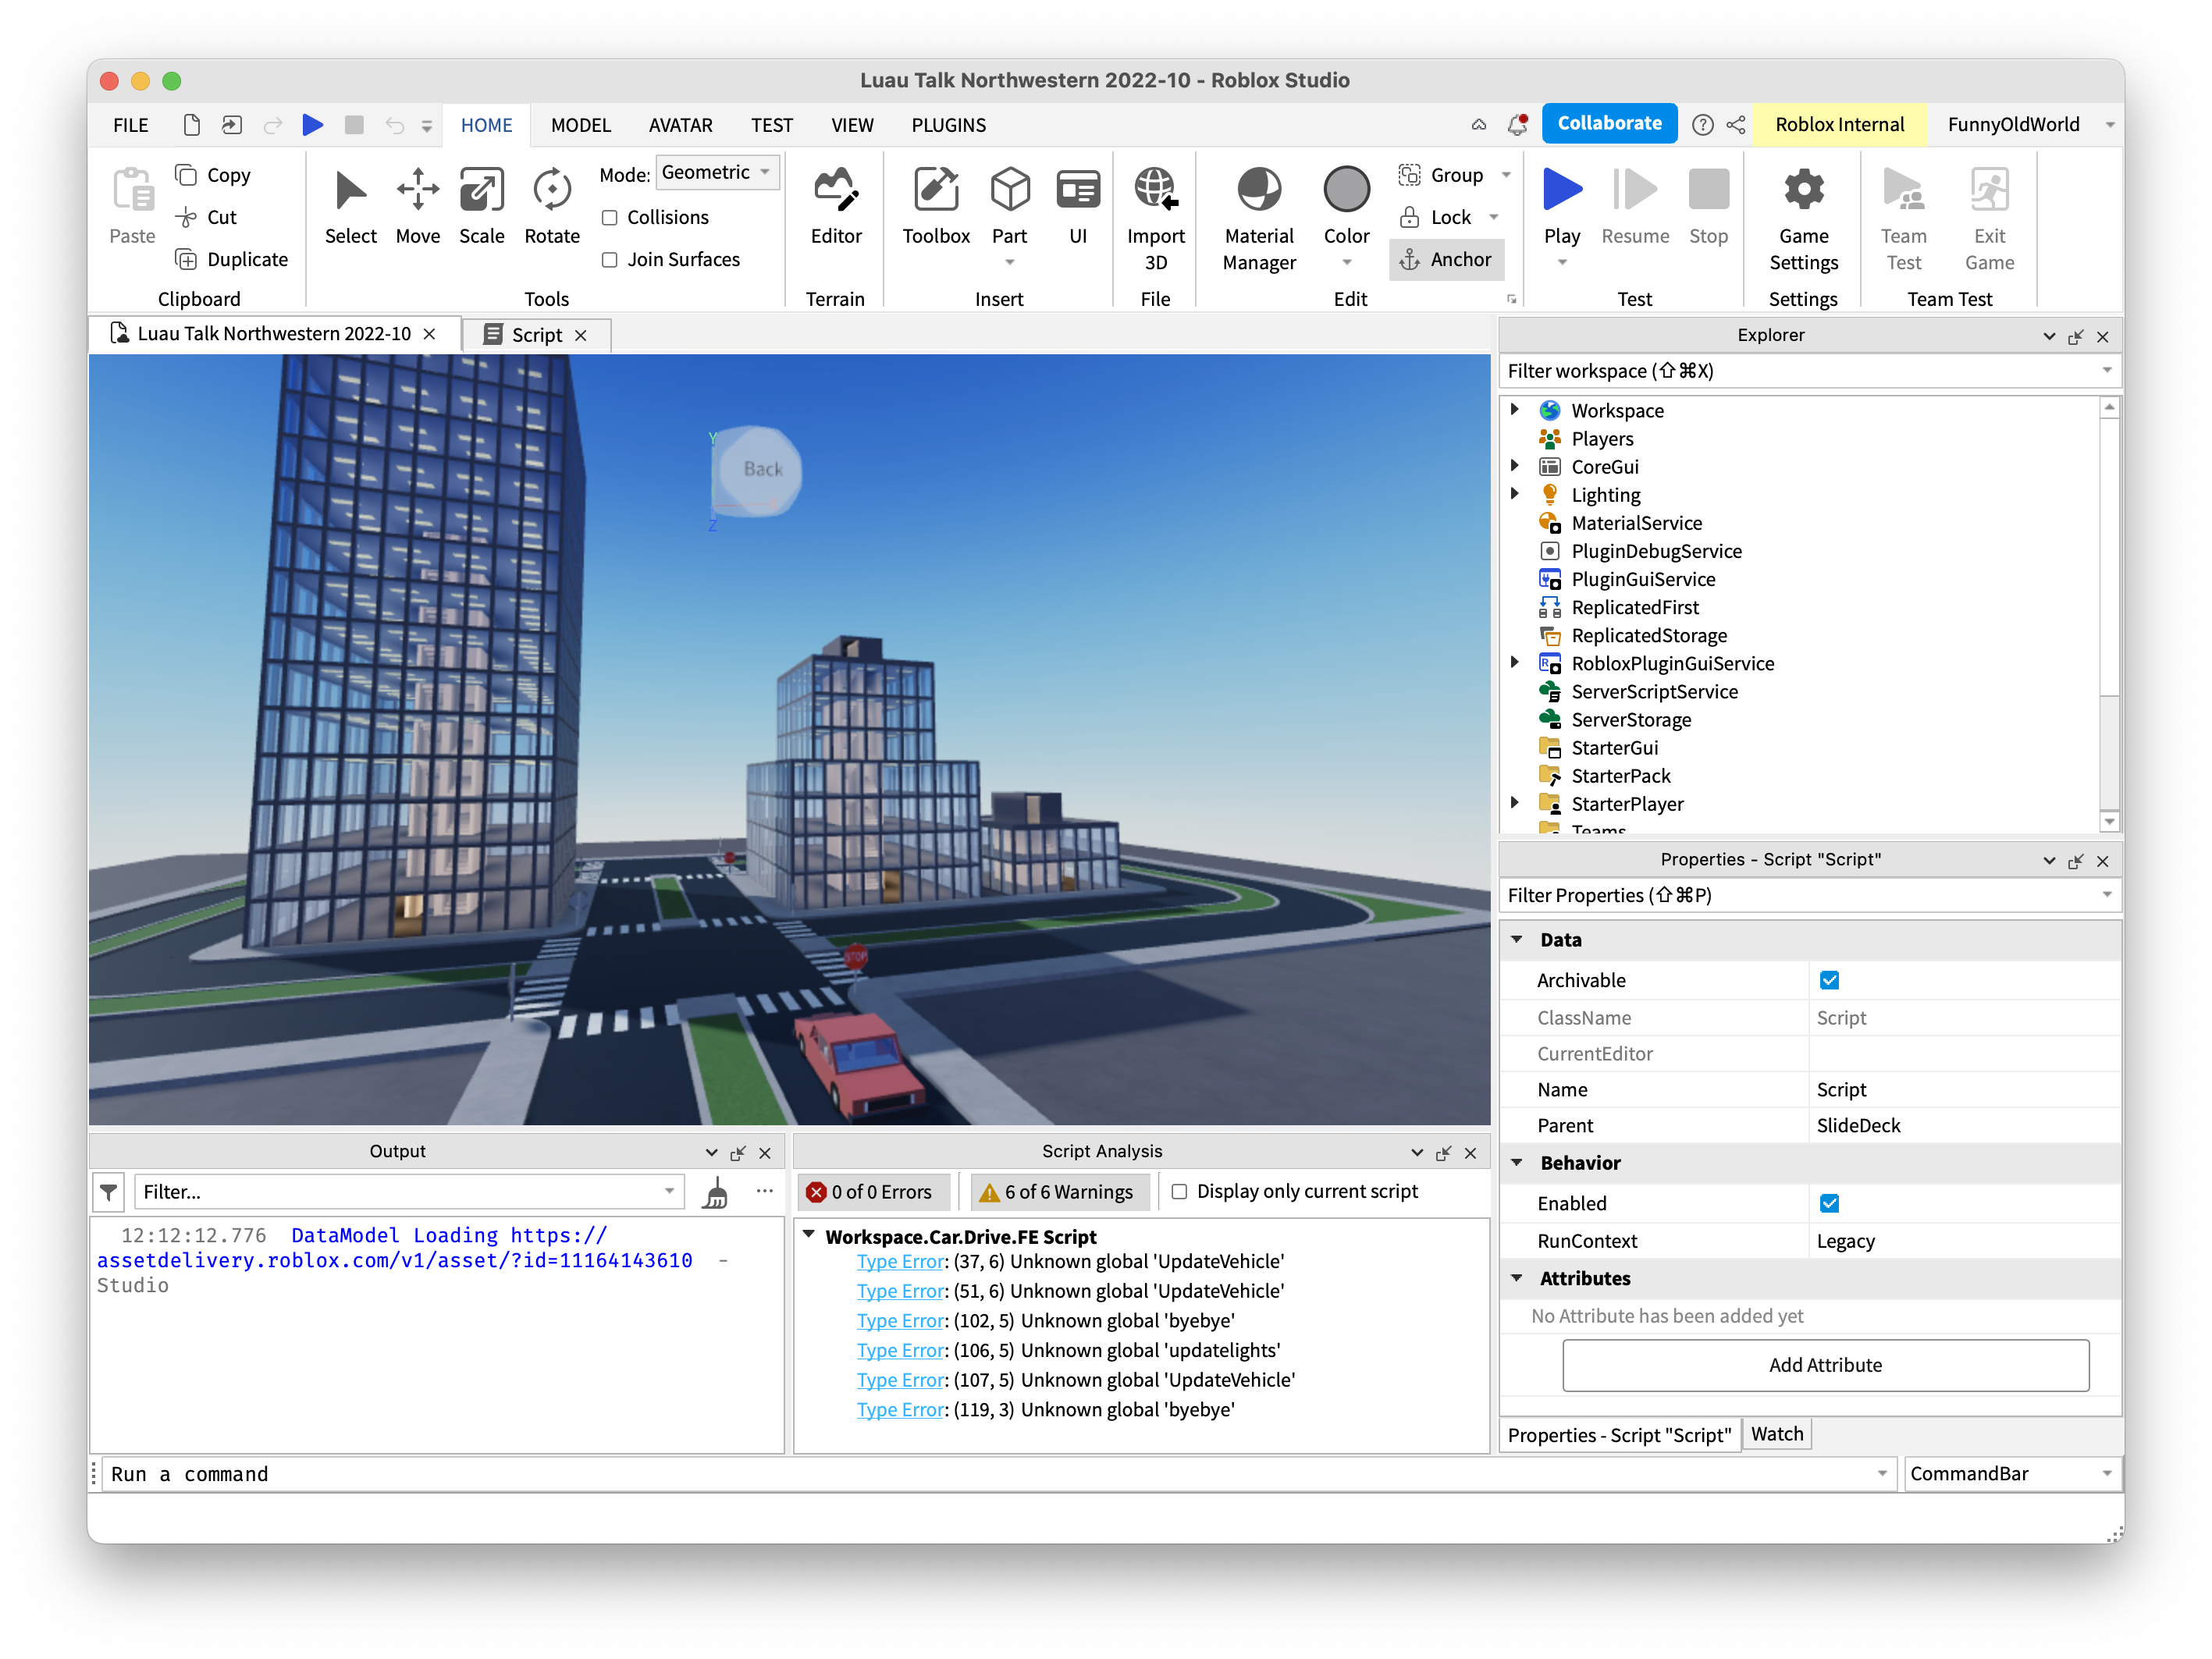
\includegraphics[width=.45\textwidth]{img/roblox-studio.png}
    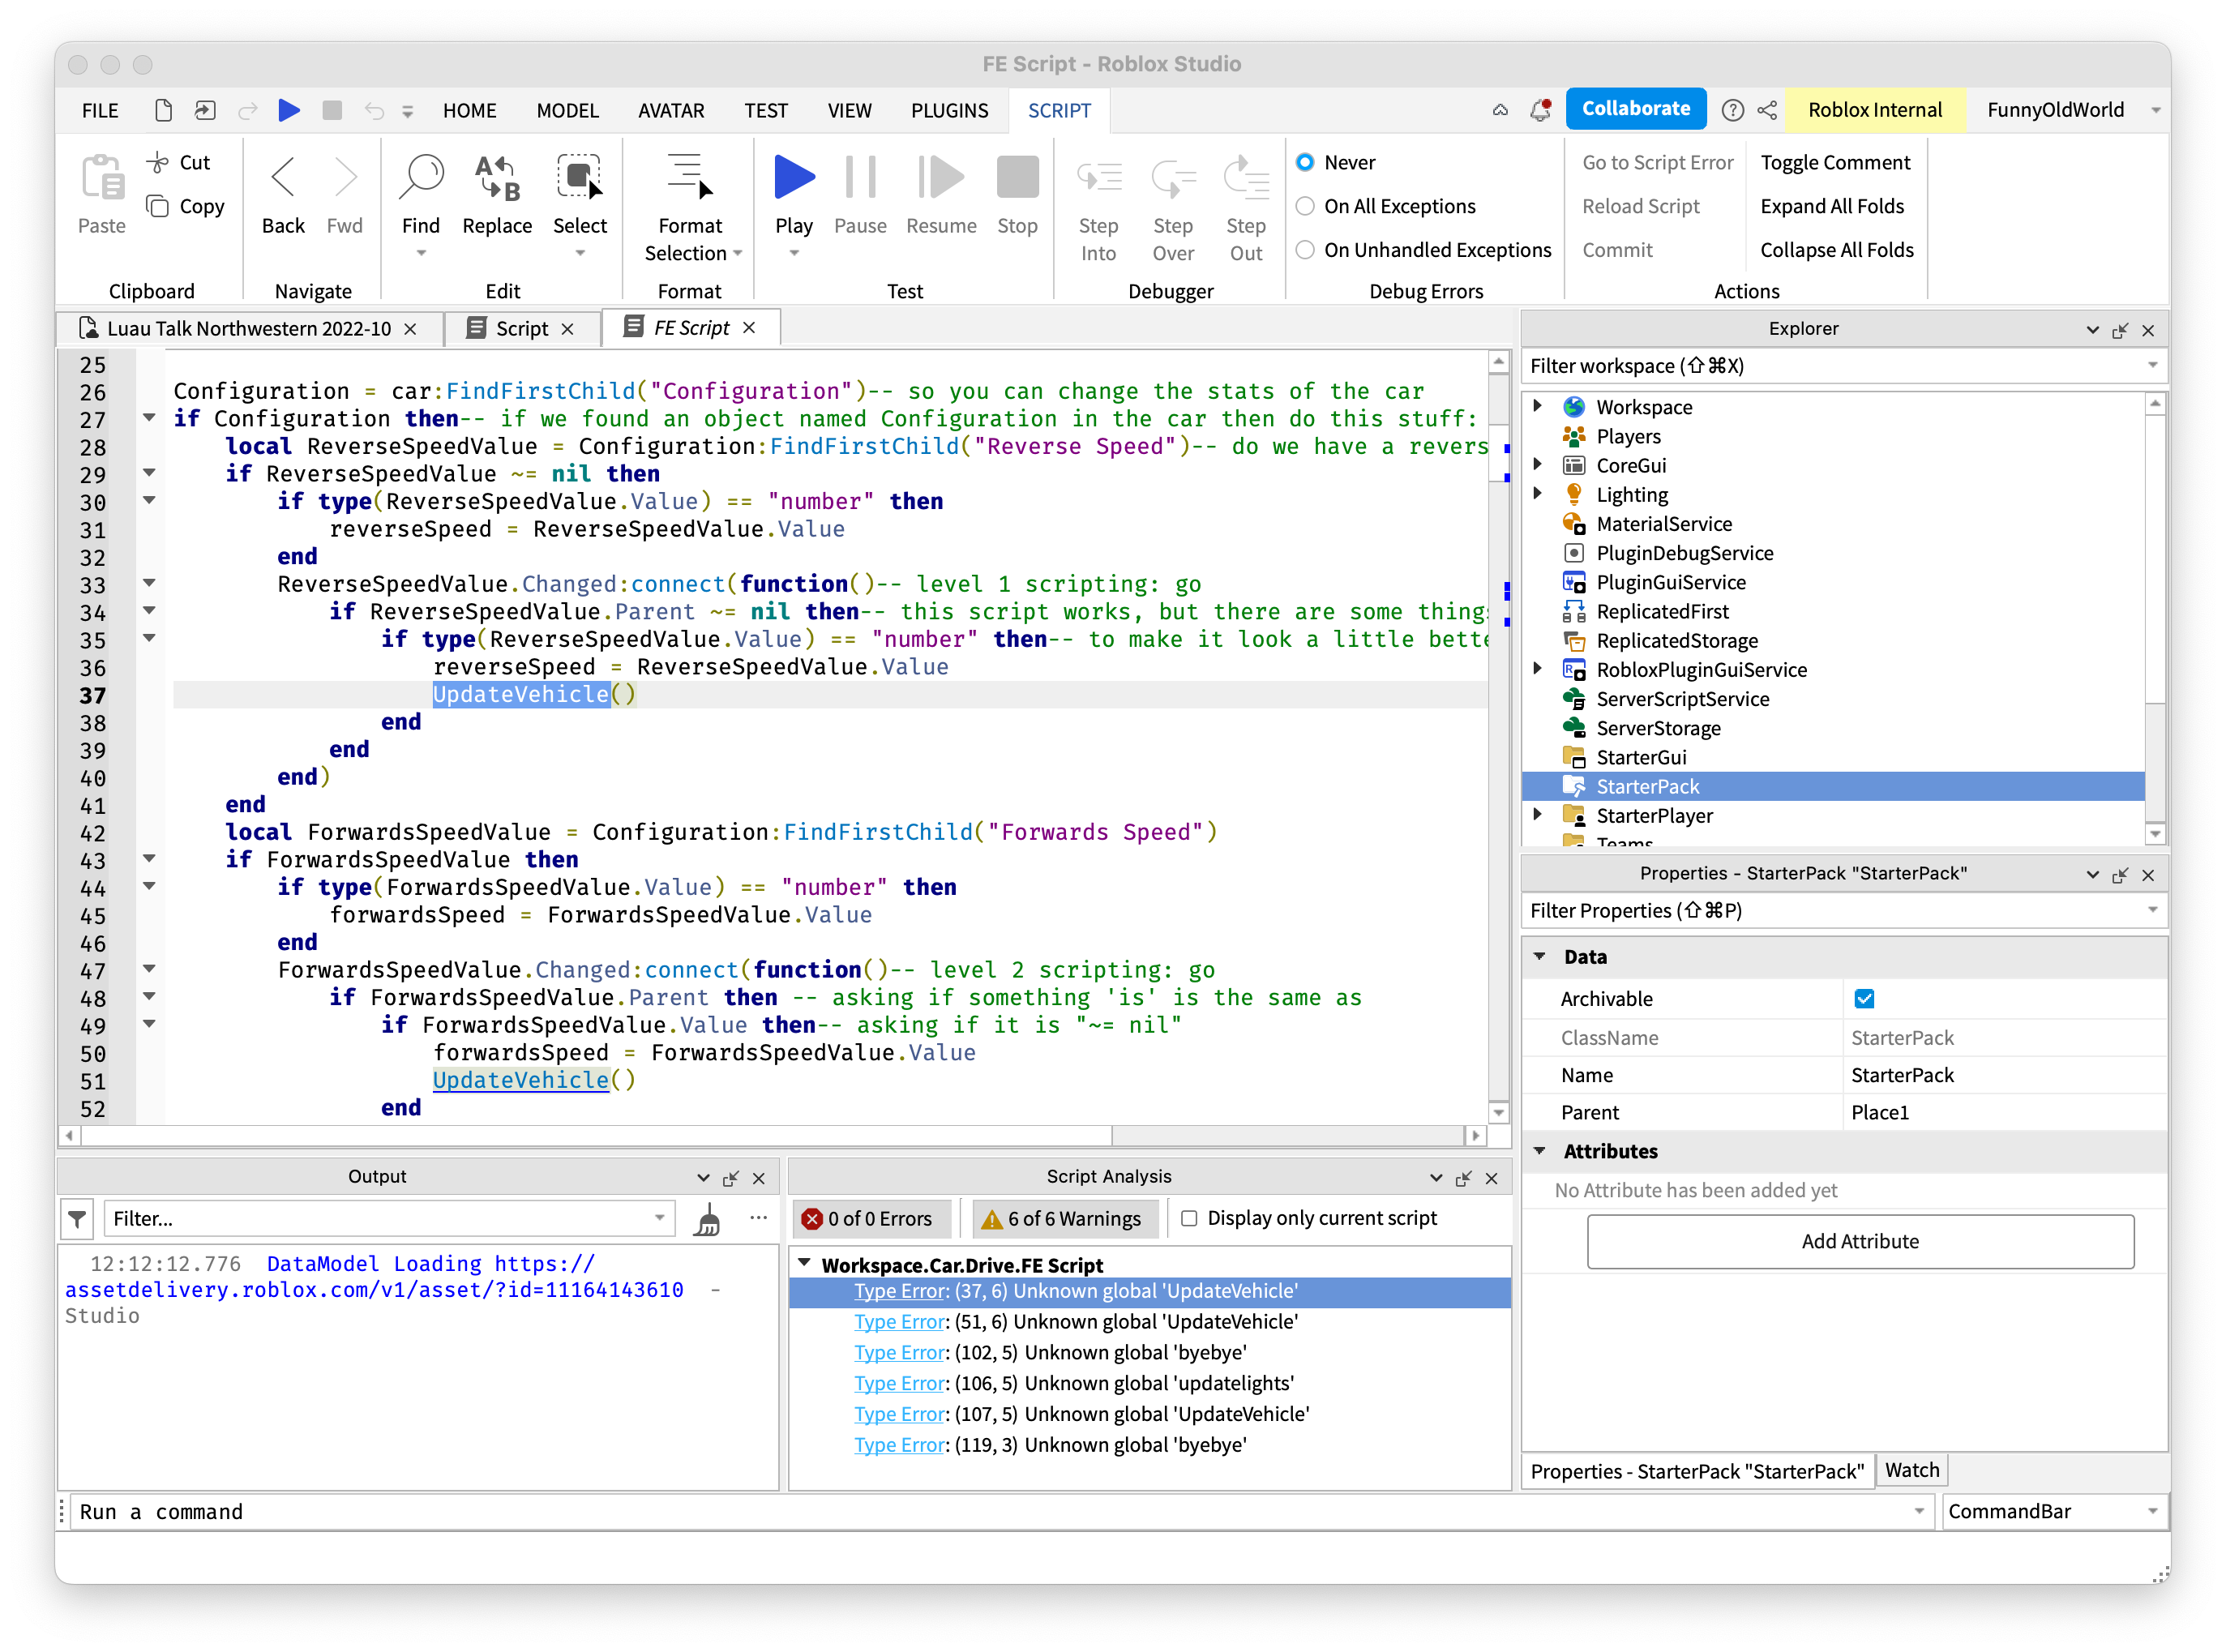
\includegraphics[width=.45\textwidth]{img/roblox-studio-ide.png}
  }
  \caption{\anon{Roblox Studio 3D creation} tools (left) and IDE (right)}
  \label{fig:roblox-studio}
\end{figure}
      
Creators of \anon{Roblox experiences} use \anon{Roblox Studio},
which combines \anon{3D creation} tools as well as an Integrated
Developer Environment (IDE), as seen in Fig.~\ref{fig:roblox-studio}.

\paragraph{Creating Experiences}

more than games

telemetry gets a session id per experience


\paragraph{Script, Module}

%% https://create.roblox.com/docs/education/coding-6/intro-to-module-scripts

script = code that runs, can have many scripts in a codebase

module = library, reusable functions, doesn't run directly

scripts are fine for basic games. professional developers are much more likely to use modules.


\paragraph{Data Model}

changes to DM can give huge type error changes

moving (re-parent) a node changes the type of the DM, unsoundness in type system

type checker assumes initial state


\section{Telemetry Design}

No PII whatsoever

Random session selection

Random events during session, except module switch.

No access to other key events: save, exit.
Don't want access to run, publish.

\url{https://docs.google.com/document/d/1DnKvw8x1jy0EWCbBSM8neKULWz7WAg1OauKy7qqYqkI/edit}


\section{Predictions}
%%bg: merge with prev section, on telemetry design?

nocheck forcestrict keep growing

nonstrict te tend to zero, fixing your program should fix the errors, no false positives

nonstrict fs unclear


\section{Results}
\label{s:data}

\begin{figure}[t]
  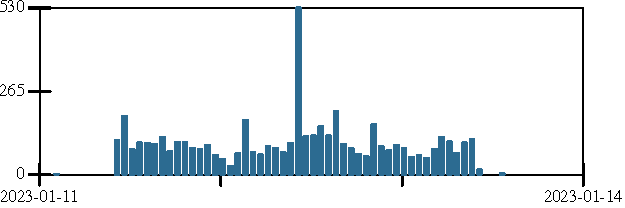
\includegraphics{img/row-distribution.pdf}
  \Description{TBD: histogram with about 100 records per hour except for a 600-record spike near the end of Jan 12th.}
  \caption{Telemetry records per hour. Each tick on the $x$-axis marks the start of a new day in California.}
  \label{f:records-per-hour}
\end{figure}

\Cref{f:records-per-hour} shows when data arrived across the whole dataset.

\begin{table}[t]
  \caption{Dataset overview}
  \label{t:dataset-overview}
\begin{tabular}{rl}
 5,108 & total logs \\
       & 4,574 nocheck + 510 nonstrict + 24 strict \\
 182,247 & total forced strict type errors \\
       & {113,274 in module, 6,425 in edit regions} \\
  1,521 & total type errors \\
       & {1,485 in module, 331 in edit regions}
  \\[2ex]

  1,146 & sessions \\
  & \begin{tabular}{rl}
      1,143 & single mode = 1046 nocheck + 94 nonstrict + 3 strict \\
      7 & multi mode projects \\
      3 & mode upgrades \\
      4 & mode downgrades
    \end{tabular}
\end{tabular}
\end{table}


\section{Interpretation}

Error 1000 = type mismatch (subtyping etc);
1001 = unknown symbol;
\ldots

% https://github.com/Roblox/luau/blob/master/Analysis/include/Luau/Error.h


\begin{verbatim}
 require(foobar)
  foobar is a module script in the data model
 require(foo.bar.b)
  - could be edit in progress
  - could be renamed module
  - 
\end{verbatim}



\section{Related Work}
\label{s:related}

\paragraph{Research on Errors}

Mind your language~\cite{mfk-onward-2011}.


\paragraph{Telemetry}

Transparent telemetry: explain what it is and contrast our approach.
What essential, non-transparent things did we collect?

TT =
no user ID, no machine ID,
no time-ordered traces,
public process to decide what to collect

https://research.swtch.com/telemetry-intro


\section{Discussion}
\label{s:conclusion}
\label{s:discussion}



\begin{acks}
  TBD

Greenman was supported by
  \grantsponsor{NSF}{NSF}{https://www.nsf.gov} grant
 \href{"https://www.nsf.gov/awardsearch/showAward?AWD_ID=2030859"}{\grantnum{NSF}{CCF 2030859}}
  to the CRA for the \href{https://cifellows2020.org}{CIFellows} project.
\end{acks}

\bibliographystyle{ACM-Reference-Format}
\bibliography{bib}

\end{document}
\endinput
